%%!TEX root = ./marylie.tex
%%--.----1----.----2----.----3----.----4----.----5----.----6----.----7----.-!

\chapter{Brief Summary of Theoretical Tools}

\section{Introduction}

     The mathematical formalism of \Mary is based on the theory of Lie
algebras and symplectic mappings.  Since these methods are new, and
probably unfamiliar, the purpose of this section is to introduce these
methods and describe how they are used in beam transport calculations.

     This chapter is organized in the following manner:

\contentsline {section}{\numberline {3.2}Hamiltonian Dynamics}{\pageref{hamiltonian}}
\contentsline {section}{\numberline {3.3}Poisson Brackets}{\pageref{poisson}}
\contentsline {section}{\numberline {3.4}Transfer Maps}{\pageref{transfer}}
\contentsline {section}{\numberline {3.5}The Symplectic Condition}{\pageref{symplectic}}
\contentsline {section}{\numberline {3.6}Taylor Expansions}{\pageref{taylor}}
\contentsline {section}{\numberline {3.7}Overview of the Lie Algebraic Approach}{\pageref{overview}}
\contentsline {section}{\numberline {3.8}Lie Operators and Lie Transformations}{\pageref{lieop}}
\contentsline {section}{\numberline {3.9}The Factorization Theorem}{\pageref{factorization}}
\contentsline {section}{\numberline {3.10}Polynomial Labeling Scheme}{\pageref{polynomial}}
\contentsline {section}{\numberline {3.11}Ingredients of a Lie Algebraic Code}{\pageref{ingredients}}
\vspace{7mm}
     In the first few subsections we show how the motion of dynamical
systems may be described in terms of certain mappings.  Then we introduce
certain Lie algebraic tools that can be used to represent these mappings.
Finally, we show how these methods are applied to beam transport
calculations.


\section{Hamiltonian Dynamics}
\label{hamiltonian}
     Consider a particle in an electromagnetic field.  We can describe its
motion using Hamilton's Equations.  Let $({\bf q},{\bf p}) = (q_1,q_2,q_3,p_1,p_2,p_3)$ denote
the generalized coordinates and momenta of the particle.  Then, for a given
set of initial conditions, the particle's subsequent motion is uniquely
determined by {\em Hamilton's Equations}:\index{Hamilton's Equations}

\begin{equation}
\begin{array}{llll}
	      {\displaystyle  \frac{dq_i}{dt}} & =  & {\displaystyle \frac{\partial H}{\partial p_i}} & (i=1,2,3), \\
	      \\
      {\displaystyle  \frac{dp_i}{dt}} & = & - {\displaystyle \frac{\partial H}{\partial q_i}} & (i=1,2,3),
\end{array}
\end{equation}
where $H({\bf q},{\bf p},t)$ is the Hamiltonian of the system.  In cartesian
coordinates $(x,y,z)$, for example, the Hamiltonian is given by the
expression
\begin{eqnarray}
\lefteqn{H(x,y,z,p_x,p_y,p_z ;t) =} \nonumber \\
 & & \sqrt{m^2 c^4 + c^2 [(p_x -qA_x)^2 + (p_y - qA_y)^2 + (p_z - qA_z)^2]} + q\phi .
\end{eqnarray}
Here ${\bf A}$ and $\phi$ are the vector and scalar potentials, respectively, and $m$  and
$q$ are the rest mass and charge of the particle, respectively.

     Now consider the passage of a particle through a beam-line element, as
shown in figure 3.2.1.  Here, the design orbit is along the $z$-axis of a
cartesian coordinate system.  When designing an accelerator, it is more
important to know when a particle will reach a particular location, and
what its transverse displacement and momentum will be there, rather than to
know its coordinates and momenta at an arbitrary time.  Referring to figure
3.2.1, one would like to know the quantities $(x,y,p_x,p_y,t)$ as functions of $z$.\index{orbit} \index{design orbit}

\begin{figure}[p]
  \centering
  \includegraphics[angle=90,scale=0.453]{beamline-passage}
  \caption{Passage Through a Beamline Element}
\end{figure}

     In many instances it is possible to choose a coordinate as an
independent variable in place of the time.  The time, in turn, is treated
as a coordinate. Finally, one introduces a momentum $p_t$ conjugate to the
time.  When this is done, say for the beam-line element of figure 3.2.1, one
automatically obtains the quantities $(x,y,t,p_x,p_y,p_t)$ as functions of $z$.

     In particular, one can find a new Hamiltonian, $K(x,y,t,p_x,p_y,p_t ;z)$,
such that the equations of motion with $z$ as an independent variable have
the form

     \begin{equation}
     \begin{array}{lllllll}
      x' &= &{\displaystyle \frac{\partial K}{\partial p_x}} & , &
p_x'& = &-{\displaystyle \frac{\partial K}{\partial x}}, \\
\\
      y' &= &{\displaystyle \frac{\partial K}{\partial p_y}} & , &
p_y'& = &-{\displaystyle \frac{\partial K}{\partial y}}, \\
\\
      t' &= &{\displaystyle \frac{\partial K}{\partial p_t}} & , &
p_t'& = &-{\displaystyle\frac{\partial K}{\partial t}}.
     \end{array}
     \end{equation}
Here, a prime denotes differentiation with respect to $z$.  Proof that such a
procedure is possible and the method for finding $K$ may be found in papers
listed in Chapter 11.  There it is also shown
that $p_t$ is the negative of the total energy,
 \begin{equation}
                           p_t  = - E.
 \end{equation}

      In most of what follows, we shall, out of convenience, speak in terms
of ``ordinary'' coordinates and momenta that are functions of time.  It
should be remembered, however, that these results are equally valid (with
the appropriate change in notation) when a {\em coordinate} is the independent
variable. Thus, when we speak of ``following a particle from some initial
time $t^{\mbox{\scriptsize in}}$ to some final time $t^{\mbox{\scriptsize fin}}$ '', the application of \Mary will actually
be in terms of ``following a particle from some initial coordinate
$z^{\mbox{\scriptsize in}}$  to some final coordinate $z^{\mbox{\scriptsize fin}}$ ''.  This will be stated explicitly in important
results.  For now, the reader should keep this at the back of his or her
mind, but not worry about it.

\section{Poisson Brackets}
\label{poisson}
    A key tool in the Lie algebraic method is the {\em Poisson bracket}.\index{Poisson bracket}  In
order to describe the Poisson bracket, and to establish terminology, it is
useful to pause for a few definitions.

\begin{quote}
         {\bf Definition}:  The six dimensional space of vectors
$({\bf q},{\bf p})$ is called
         {\em phase space}.  The variables $q_i$  and $p_i, (i = 1,2,3)$ are  called
         {\em phase-space variables}.  A {\em dynamical variable},
$f({\bf q},{\bf p})$, is
         any smooth function of the phase space variables.  (Note that  $H$,
         $q_i$ and $p_i$  are all dynamical variables.)  Since the only  functions
         we shall be concerned with are also dynamical variables, we shall
         use ``function'' and ``dynamical variable''  interchangeably.
\end{quote}
\index{phase space}

     The Poisson bracket arises naturally when we consider the time rate of
change of a dynamical variable $f$ along a trajectory.  By the chain rule, we
have the relation
\begin{equation}
       (\frac{d\ }{dt}) f({\bf q},{\bf p}) =  \sum_{i=1}^3  \frac{\partial f}{\partial q_i} \dot{q}_i  + \frac{\partial f}{\partial p_i} \dot{p}_i .
\end{equation}
Using Hamilton's equations (3.2.1), this becomes
\begin{equation}
             \frac{df}{dt} =  \sum_{i=1}^3 \frac{\partial f}{\partial q_i} \frac{\partial H}{\partial p_i} - \frac{\partial f}{\partial p_i} \frac{\partial H}{\partial q_{i}}.
\end{equation}
Now introduce the Poisson bracket $[f,g]$ of any two functions $f$ and $g$.  It
is defined by the rule
\begin{equation}
         [f,g]  \stackrel{\rm def}{=}  \sum_{i=1}^3 \frac{\partial f}{\partial q_i} \frac{\partial g}{\partial p_i} - \frac{\partial f}{\partial p_i} \frac{\partial g}{\partial q_i}.
\end{equation}
Then (3.3.2) can be written in the more compact form
\begin{equation}
                     \frac{df}{dt} = [f,H].
\end{equation}
Note that Hamilton's equations (3.2.1) can be written as a special case of
(3.3.4),
\begin{equation}
         \frac{dq_i}{dt}  = [q_i,H]
\end{equation}
\begin{equation}
         \frac{dp_i}{dt}  = [p_i,H].
\end{equation}

\section{Transfer Maps}
\label{transfer}
     For convenience of discussion, it is useful to employ a notation that
treats coordinates and momenta on an equal footing.  To this end, let
${\bf z}$
denote the vector with six entries given by the rule
\begin{equation}
     {\bf z} = ({\bf q},{\bf p}) = (q_1,q_2,q_3,p_1,p_2,p_3).
\end{equation}
(Note that here, and generally from now on, the symbol $z$ has a different
meaning than in section 3.2.)  Hamilton's equations can now be written in
the compact form
\begin{equation}
            \frac{d{\bf z}}{dt} = -[H,{\bf z}\,] .
\end{equation}

     Next, consider the 7-dimensional space consisting of ${\bf z}$ and $t$.  We call this
{\em augmented phase space}.\index{augmented phase space}  Suppose a particle has initial phase-space
coordinates ${\bf z}^{\mbox{\scriptsize \ in}}$   at
some initial time $t^{\mbox{\scriptsize in}}$.  This state of affairs is represented by the point
$({\bf z}^{\mbox{\scriptsize \ in}},t^{\mbox{\scriptsize in}})$ in augmented phase space.  As the particle moves (in accord with Hamilton's
equations), the vector $({\bf z},t)$ will trace out a trajectory in the augmented phase space.
See figure 3.4.1.

\begin{figure}[h]
  \centering
  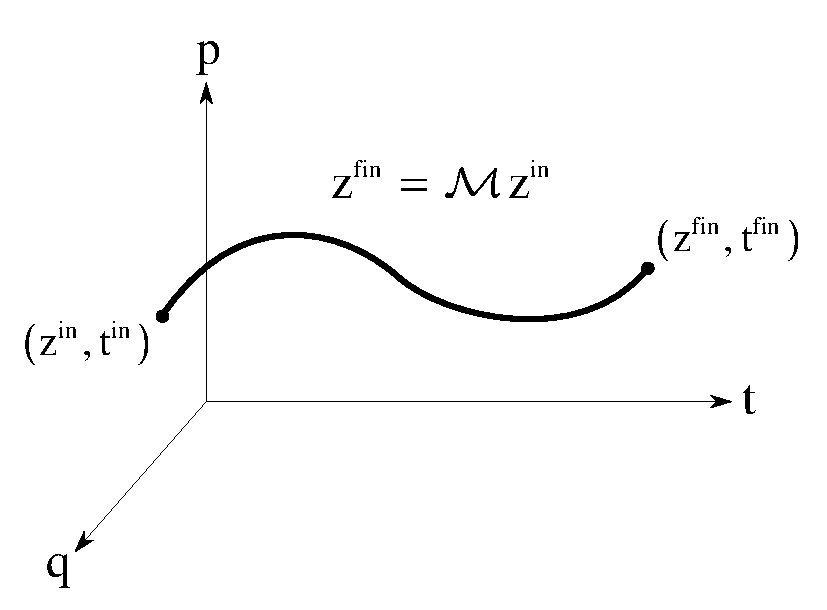
\includegraphics{statespace}
  \caption{Augmented Phase Space}
\end{figure}


     Now let the time $t^{\mbox{\scriptsize in}}$ be fixed.  By
specifying initial conditions ${\bf z}^{\mbox{\scriptsize \ in}}$,
we also specify a unique trajectory since every point in augmented phase space has
exactly one trajectory passing through it.  We can follow this trajectory
to some final time, $t^{\mbox{\scriptsize fin}}$   .  We can also do this for every other trajectory
starting at $t^{\mbox{\scriptsize in}}$  .  The set of all trajectories so obtained is called the {\em Hamiltonian flow}\index{Hamiltonian flow} (between $t^{\mbox{\scriptsize in}}$   and $t^{\mbox{\scriptsize fin}}$).

     We can, of course, also reverse this procedure.  Any point (${\bf z}^{\mbox{\scriptsize \ fin}}$, $t^{\mbox{\scriptsize fin}}$)
may be followed backward in time to some point (${\bf z}^{\mbox{\scriptsize \ in}}$, $t^{\mbox{\scriptsize in}}$).  Since the
correspondence between ${\bf z}^{\mbox{\scriptsize\ in}}$ and ${\bf z}^{\mbox{\scriptsize \ fin}}$    is one to one, we may regard them as
being related by some invertible (generally nonlinear) map ${\cal M}$.  We write,
symbolically,
\begin{equation}
      {\bf z}^{\mbox{\scriptsize \ fin}}  = {\cal M} {\bf z}^{\mbox{\scriptsize
      \ in}}   .
\end{equation}
We say that ${\cal M}$ is generated by ``following'' the Hamiltonian flow from $t^{\mbox{\scriptsize in}}$   to $t^{\mbox{\scriptsize fin}}$.  Since ${\cal M}$ relates initial and final conditions, it will often be
referred to as a {\em transfer map}.\index{transfer map}  In our applications, we shall utilize
transfer maps corresponding to various beamline elements.  Such mappings
relate coordinates and momenta at the exit face of an element to those at
the entrance face.


\section{The Symplectic Condition}
\label{symplectic}
     The fact that ${\cal M}$ arises from following a Hamiltonian flow imposes
strong restrictions on its nature.  Indeed, ${\cal M}$ belongs to a class of
mappings known as {\em symplectic} mappings.  Consider the Jacobian matrix $M$ that
characterizes the {\em local linear} behavior of ${\cal M}$.  It is defined by the
equations
\begin{equation}
          M_{ab}(z^{\mbox{\scriptsize in}}) = \frac{\partial z_a^{\mbox{\scriptsize fin}}}{\partial z_b^{\mbox{\scriptsize in}}}.
\end{equation}
That is, $M$ describes how small changes in the initial conditions produce
small changes in the final conditions.  Note that in general $M$ depends on
the trajectory in question, and thus we write $M(z^{\mbox{\scriptsize in}})$.  Next, define a matrix $J$, called the {\em Poisson} matrix, by the equation
\begin{equation}
           J = \left( \begin{array}{cc}
                      0 & I\\
                      -I & 0
                      \end{array}
               \right).
\end{equation}\index{J matrix}
Here each entry in $J$ is a $3 \times 3$ block, and $I$ denotes the $3 \times 3$ identity
matrix.\index{Poisson matrix}  Then it can be shown that $M$ obeys the relation
\begin{equation}
       M^T(z^{\mbox{\scriptsize in}}) J M(z^{\mbox{\scriptsize in}}) = J \mbox{ for all }z^{\mbox{\scriptsize in}}.
\end{equation}
Here $M^T$ denotes the transpose of $M $.

     Equation (3.5.3) is the condition that $M$ be a {\em symplectic} matrix.\index{symplectic matrix}
Correspondingly, a map ${\cal M}$ whose Jacobian matrix $M$ is symplectic is said to
be a {\em symplectic map}.\index{symplectic map}

     Note that the left hand side of (3.5.3) should generally depend on $z^{\mbox{\scriptsize in}}$
since $M$ depends on $z^{\mbox{\scriptsize in}}$.  By contrast, the right hand side of (3.5.3) is independent of $z^{\mbox{\scriptsize in}}$.  Consequently, ${\cal M}$ is strongly restricted by the symplectic condition.

     A proof of the symplectic condition and a discussion of some of its
consequences may be found in some of the papers listed in Chapter 11.  There it is also shown that a symplectic map is a
canonical transformation, and vice versa.\index{canonical transformation}  It is sufficient for present
purposes to say that a major reason for using Lie algebraic methods is to
exploit the symplectic condition.

Finally, we observe that for purposes of Accelerator Physics it is more convenient to employ the phase-space coordinate ordering (6.18.1) rather than (4.1).  In this case the matrix $J$ takes the form (6.18.2).

\section{Taylor Expansions}
\label{taylor}
     For most beam line elements, there is a well defined reference or
``design'' trajectory.  For example, the design trajectory for a quadrupole
magnet is the trajectory running along its axis.  Suppose we choose our
phase-space coordinate systems at $t^{\mbox{\scriptsize in}}$ and $t^{\mbox{\scriptsize fin}}$ in such a way that the
design trajectory has ${\bf z}^{\mbox{\scriptsize \ in}} = 0$ and ${\bf z}^{\mbox{\scriptsize \ fin}} = 0$.  Then, for orbits near the
design orbit, ${\bf z}^{\mbox{\scriptsize \ in}}$ and
${\bf z}^{\mbox{\scriptsize \ fin}}$ are small.  In this case we may expand the
relation between ${\bf z}^{\mbox{\scriptsize \ fin}}$ and
${\bf z}^{\mbox{\scriptsize \ in}}$, given symbolically by (3.4.3), in a more
concrete series representation.\index{Taylor expansion}  We write
\begin{equation}
z_a^{\mbox{\scriptsize fin}} = \sum_b R_{ab} z_b^{\mbox{\scriptsize in}} +
\sum_{b,c} T_{abc} z_b^{\mbox{\scriptsize in}} z_c^{\mbox{\scriptsize in}} +
       \sum_{b,c,d} U_{abcd} z_b^{\mbox{\scriptsize in}} z_c^{\mbox{\scriptsize in}} z_d^{\mbox{\scriptsize in}} + \cdots .
\end{equation}
Here $R$ is the usual transfer matrix of linear matrix theory, and $T$ is the
second order transfer matrix, as calculated in the commonly used code
TRANSPORT.  The quantities $U$ describe third order corrections, and are not
usually treated by present codes.\index{transfer matrix}  Third order contributions are, however,
handled routinely by \Mary 3.0.\index{R matrix} \index{T matrix} \index{U matrix}

     Because ${\cal M}$ is a symplectic map, the various quantities $R, T, U, \ldots$ are
not all independent.  Instead, they are interrelated as a result of (3.5.3)
by rather complicated linear and nonlinear equations.  Moreover, it can be
shown that in general the series (3.6.1) cannot be truncated without
violating the symplectic condition.  Consequently, the use of truncated
Taylor series does not lead to an approximation scheme that is consistent
with the symplectic condition.  For these reasons, (3.6.1) is usually not the best way to
parameterize a symplectic transfer map.

\section{Overview of the Lie Algebraic Approach}
\label{overview}
     We have seen that the motion of a charged particle through a beam line
element can be described by a symplectic transfer map ${\cal M}$.  The Lie algebraic
approach provides tools for representing such maps, and for combining
symplectic maps for individual elements to find grand maps for collections
of beam line elements.

     First, we will show that given any dynamical variable $f$, we can use
the Poisson bracket to obtain an associated operator, which we shall denote
by the symbols $\Lieop(f)$.  These operators are called {\em Lie operators}.  (We will also refer to $f$ as a {\em Lie generator}.)\index{Lie generator} \index{generator}  Next we
will describe how symplectic maps ${\cal M}$ can be written down and manipulated in
terms of Lie operators.  Finally, we will indicate how the symplectic maps
for various beam line elements and collections of beam line elements can be
described in terms of various polynomials.

\section{Lie Operators and Lie Transformations}\index{operator}
\label{lieop}
     Suppose $f$ is some function of the phase-space variables $z$.  Associated
with every such function will be a {\em Lie operator} denoted by
$\Lieop(f)$.\index{Lie operator}  The Lie
operator $\Lieop(f)$ is a {\em differential} operator defined by the rule
\begin{equation}
           \Lieop(f) \ \stackrel{\rm def}{=} \sum_i (\partial f/\partial
		   q_i) (\partial /\partial p_i) - (\partial f/\partial p_i)(\partial
		   /\partial q_i).
\end{equation}
In particular, if $\Lieop(f)$ acts on any phase-space function $g$, one
finds the result
\begin{equation}
           \Lieop(f)g = \sum_i (\partial f/\partial
		   q_i) (\partial g/\partial p_i) - (\partial f/\partial p_i)(\partial
		   g/\partial q_i) = [f,g].
\end{equation}
Thus, one may heuristically view a Lie operator as a Poisson bracket
waiting to happen.

     Now that Lie operators have been defined, it is a simple matter to
define powers of Lie operators.  Powers are defined in terms of multiple
Poisson brackets:
\begin{equation}
\begin{array}{c}
           {\Lieop(f)}^0 g = g,\\
                         \\
           {\Lieop(f)}^1 g = [f,g],\\
                             \\
           {\Lieop(f)}^2 g = \Lieop(f)\:\Lieop(f)g = [f,[f,g]],\\
                                           \\
           {\Lieop(f)}^3 g = [f,[f,[f,g]]], {\rm etc.}\\
\end{array}
\end{equation}

     Next we define the {\em exponential} of a Lie operator $\Lieop(f)$ by writing the
series
\begin{equation}
       e^{:f:} = \exp (:f:) \stackrel{\rm def}{=} \sum_{m=0}^{\infty} \frac{{\Lieop(f)}^m}{m!}.
\end{equation}
The quantity $e^{:f:}$ or $\exp (:f:)$ will be called the {\em Lie transformation }\index{Lie transformation} associated with
$f$.  We shall be concerned primarily with the operation of $e^{:f:}$ on each
component $z_a$.  In accord with the definitions (3.8.3) and (3.8.4), we have
the relation
\begin{equation}
      e^{:f:} z_a = z_a + [f,z_a] + \frac{[f,[f,z_a]]}{2!} + \cdots.
\end{equation}

     Lie operators and Lie transformations have a number of important
properties that are described in detail in some of the papers listed
in Chapter 11.  One basic property worth noting here is that, in
general, Lie operators do not commute,
\begin{equation}
      \Lieop(f)\:\Lieop(g) \neq \Lieop(g)\:\Lieop(f).
\end{equation}
Indeed, one can prove the relation
\begin{equation}
      \Lieop(f)\:\Lieop(g) - \Lieop(g)\:\Lieop(f) = \Lieop([f,g]).
\end{equation}
Consequently, the commutator of two Lie operators can be computed in terms
of Poisson brackets.

     As a result of the noncommutativity of Lie operators, Lie
transformations also do not commute in general; nor do their exponents
generally add:
\begin{equation}
\begin{array}{lll}
                  e^{:f:} e^{:g:} & \neq & e^{:g:} e^{:f:},\\
                                  &      &                 \\
                  e^{:f:} e^{:g:} & \neq & e^{(:f: + :g:)}.
\end{array}
\end{equation}

\section{Factorization Theorem}
\label{factorization}
     The importance of Lie operators and Lie transformations for our
present purposes is a consequence of the {\em factorization theorem}.\index{factorization theorem}  This
theorem states that symplectic maps can be written in terms of products of
Lie transformations, and these Lie transformations are of a very simple
kind.

     Suppose ${\cal M}$ is a symplectic map of the form (3.6.1).  Then ${\cal M}$ can be
represented as an infinite product of Lie transformations,
\begin{equation}
      {\cal M} = e^{:f_2:} e^{:f_3:} e^{:f_4:} \cdots.
\end{equation}
Here each function $f_n$ is a {\em homogeneous polynomial} of degree
$n$ in the phase-space variables ${\bf z}^{\mbox{\scriptsize \ in}}$.

     There are a number of important features of the factored product
representation.  Those of particular interest for our present concerns are
listed below.  More detailed discussion may be found in some of the papers
listed in Chapter 11.

\begin{itemize}
  \item  Any set of homogeneous polynomials $f_n$,  when employed in  (3.9.1),
         will produce a symplectic map.  Thus, the restrictions  imposed on
         ${\cal M}$ by the symplectic condition are automatically  taken care of by
         the use of Lie transformations.

  \item  As a corollary of the previous statement, it follows that the
         infinite product (3.9.1) can be truncated at any stage, and the
         result is still a symplectic map.

  \item  Suppose we compare the representations (3.6.1) and (3.9.1).
         Then, as will be shown shortly, one finds that $R$ is completely
         specified in terms of $f_2$.  Also, $T$ is completely specified in
         terms of $f_3$.  Finally, $U$ is completely specified in terms of $f_3$
         and $f_4$.  Thus if one is content with results that are correct
         through third order, as explicitly displayed in (3.6.1), then  one
         only need work with polynomials $f_2$, $f_3$, and $f_4$  in (3.9.1).   A
         count shows that there are 203 (linearly independent) such
         polynomials in six variables.  By contrast, if we count the
         number of parameters involved in $R$, $T$, and $U$ (when the  symplectic
         condition is overlooked), we find that this number  is much
         larger.  Thus, the use of Lie algebraic methods requires
         considerably less computer storage. \index{R matrix} \index{T matrix} \index{U matrix}

In summary, the factor $\exp (:f_2:)$ describes the {\em linear} part \index{linear part} of ${\cal M}$, and the remaining factors $\exp (:f_3:)$ $\exp (:f_4:)$ $\cdots$ describe the {\em nonlinear} part \index{nonlinear part}

  \item  As may be inferred from the previous discussion, each $f_n$  has a
         direct physical interpretation.  For example, second order
         effects due to sextupole magnets are described by $f_3$.  Third
         order effects due to octupole magnets and iterated sextupoles  are
         described by $f_4$.  Were one to include fourth and fifth order
         effects, as is envisioned for example for \Mary 5.0, then one
         only need adjoin the homogeneous polynomials $f_5$  and $f_6$.
\end{itemize}

     As an illustration for the reader of some aspects of Lie algebraic
calculations, we will verify the statements made in the third item above.  Consider
the evaluation of
\begin{eqnarray}
    e^{:f_2:} z_a & = & z_a + \Lieop(f_2) z_a + \frac{{\Lieop(f_2)}^{2} z_a}{2!} + \cdots \nonumber \\
                        &   & \nonumber \\
                        & = & z_a + [f_2,z_a] + \frac{[f_2,[f_2,z_a]]}{2!} +
\end{eqnarray}
We know that, by definition, $f_2$  is of degree 2.  What are
the degrees of the terms $[f_2,z_a]$, $[f_2,[f_2,z_a]]$, etc.?
Inspection of the Poisson bracket operation (3.3.3) shows that it contains two
differentiations. Consequently, $[f_2,z_a]$ must be of degree one.  Since
$[f_2,z_a]$ is of degree one, it follows that $[f_2,[f_2,z_a]]$ must
also be of degree one, etc.  We conclude that all the terms on the right hand
side of (3.9.2) are of degree one.  Therefore (3.9.2) is a linear
transformation, and there exist coefficients $R_{ab}$   such that
\begin{equation}
       e^{:f_2:} z_a^{\mbox{\scriptsize in}}   = \sum_b R_{ab} z_b^{\mbox{\scriptsize in}}.
\end{equation}

     Next consider the evaluation of
\begin{eqnarray}
  e^{:f_n:} z_a^{\mbox{\scriptsize in}} & = & z_a^{\mbox{\scriptsize in}} + \Lieop(f_n) z_a^{\mbox{\scriptsize in}} + \frac{\Lieop(f_n)^2}{2!}z_a^{\mbox{\scriptsize in}} + \cdots \nonumber \\
 &   &  \nonumber \\
 & = & z_a^{\mbox{\scriptsize in}} + [f_n,z_a^{\mbox{\scriptsize in}}] + \frac{[f_n,[f_n,z_a^{\mbox{\scriptsize in}}]]}{2!} + \cdots,
\end{eqnarray}
where $n \geq 3$.  Suppose that $g_m$ and $g_n$  are two homogeneous polynomials of
degrees $m$ and $n$ respectively.  Then inspection of (3.3.3) shows that
$[g_m,g_n]$ is a homogeneous polynomial of degree $m+n-2$.  It follows that the
terms $[f_n,z_a], [f_n,[f_n,z_a]], \ldots$ are of degrees $n-1, 2n-3$, etc.  We see
that, provided $n \geq 3$, the terms on the right hand side of (3.9.4) are of
successively higher degree. Comparison with (3.6.1) shows that only $[f_3,z_a]$
contributes to the second order terms, and only $[f_3,[f_3,z_a]]$ and $[f_4,z_a]$
contribute to the third order terms.  We also conclude that polynomials $f_n$
of degree five and higher only contribute to terms in (3.6.1) of degree
four and higher.

\section{Polynomial Labeling Scheme}
\label{polynomial}
     As indicated in the previous section, symplectic maps ${\cal M}$ that send the
origin into itself may be specified through third order in terms of
polynomials $f_2$, $f_3$, and $f_4$.  In 6 variables, there are a fixed number of
different monomials of any given degree.\index{polynomial labeling}  The numbers of such monomials for
each degree through degree 9 are listed below:
\begin{center}
\begin{tabular}{||r|c|r||}            \hline
    \multicolumn{1}{||c}{ } &
    \multicolumn{1}{|c|}{Number of Monomials N(n) of} &
    \multicolumn{1}{c||}{ } \\
    \multicolumn{1}{||c}{Degree n} &
    \multicolumn{1}{|c|}{Degree n in 6 variables} &
    \multicolumn{1}{r||}{Running Total} \\     \hline
        1             &             6                &              6 \\
        2             &            21                &             27 \\
        3             &            56                &             83 \\
        4             &           126                &            209 \\
        5             &           252                &            461 \\
        6             &           462                &            923 \\
        7             &           792                &           1715 \\
        8             &          1287                &           3002 \\
        9             &          2002                &           5004 \\ \hline
\end{tabular}
\end{center}

     These monomials may be listed sequentially, and consequently each
monomial may be labeled by a number called its {\em index}.\index{monomial index} \index{index}  One way of doing
this is illustrated below for the first few monomials.  The variables used
are those of section 4.1.2.
\begin{center}
\begin{tabular}{ccccccc}
\multicolumn{4}{c}{ } &
\multicolumn{3}{c}{Exponents} \\
    Index   & &     Monomial  & &  $X$  $P_x$ &  $Y$  $P_y$ & $\tau$  $P_{\tau}$ \\ \cline{1-1} \cline{3-3} \cline{5-7}
      1     & &         $X$     & &  1  0 & 0  0 & 0  0 \\
      2     & &        $P_x$  & &  0  1 & 0  0 & 0  0 \\
      3     & &         $Y$     & &  0  0 & 1  0 & 0  0 \\
      4     & &        $P_y$  & &  0  0 & 0  1 & 0  0 \\
      5     & &        $\tau$   & &  0  0 & 0  0 & 1  0 \\
      6     & &      $P_{\tau}$ & &  0  0 & 0  0 & 0  1 \\
      7     & &        $X^2$  & &  2  0 & 0  0 & 0  0 \\
      8     & &       $XP_x$  & &  1  1 & 0  0 & 0  0 \\
\multicolumn{1}{c}{$\vdots$} &
\multicolumn{1}{c}{ } &
\multicolumn{1}{c}{$\vdots$} &
\multicolumn{1}{c}{ } &
\multicolumn{3}{c}{$\vdots$} \\
     26     & & $\tau P_{\tau}$ & &  0  0 & 0  0 & 1  1 \\
     27     & &  $P_{\tau}^2$ & &  0  0 & 0  0 & 0  2 \\
     28     & &      $X^3$    & &  3  0 & 0  0 & 0  0 \\
     29     & &   $X^2 P_x$ & &  2  1 & 0  0 & 0  0 \\
\multicolumn{1}{c}{$\vdots$} &
\multicolumn{1}{c}{ } &
\multicolumn{1}{c}{$\vdots$} &
\multicolumn{1}{c}{ } &
\multicolumn{3}{c}{$\vdots$} \\
     82     & & $\tau P_{\tau}^2$ & &  0  0 & 0  0 & 1  2 \\
     83     & &    $P_{\tau}^3$   & &  0  0 & 0  0 & 0  3 \\
     84     & &       $X^4$       & &  4  0 & 0  0 & 0  0 \\
     85     & &    $X^3 P_x$    & &  3  1 & 0  0 & 0  0 \\
\multicolumn{1}{c}{$\vdots$} &
\multicolumn{1}{c}{ } &
\multicolumn{1}{c}{$\vdots$} &
\multicolumn{1}{c}{ } &
\multicolumn{3}{c}{$\vdots$} \\
     208    & & $\tau P_{\tau}^3$ & &  0  0 & 0  0 & 1  3 \\
     209    & &    $P_{\tau}^4$   & &  0  0 & 0  0 & 0  4
\end{tabular}
\end{center}
This labeling is given in detail in Chapter 14 for all monomials through
degree 4.

     The indexing scheme just described is used in \Mary 3.0 to label the
monomial coefficients occurring in $f_3$  and $f_4$ .  Thus, for example, when
\Mary 3.0 is asked to print the nonlinear part of the transfer map as in
section 2.2, the quantities $f(i)$ are the nonzero coefficients of the
monomials with indices $i$ appearing in $f_3$  and $f_4$ .  Note that for the
convenience of the reader, the corresponding exponents are also displayed.

     The indices 1 through 6 corresponding to $f_1$  and the indices 7 through
27 corresponding to $f_2$ are not used by \Mary 3.0 for the specification of
transfer maps.  (They are used, however, for other purposes.  They will
also be used by \Mary 3.1 for the specification of transfer maps that do
not send  the origin into itself.)  In view of (3.9.2) and (3.9.3), $f_2$
could be used to specify the matrix part $R$ of a transfer map.  However,
according to (3.9.2), the computation of $R$ from $f_2$  requires the summation
of an infinite series.  It is therefore more convenient for most purposes
to store and manipulate the matrices $R$ directly.

\section{Ingredients of a Lie Algebraic Code}
\label{ingredients}
     The Lie algebraic concepts just sketched, and their consequences, can
be used to make a Lie algebraic charged particle beam transport code.  The
special ingredients of such a code are described briefly below.

%\numberbysubsection
\subsection{Element Library}
     We have seen that the effect of a beamline element is described by a
symplectic map, and that a symplectic map (through terms of degree three)
is described in turn by certain polynomials $f_2$, $f_3$, and $f_4$.  The first
ingredient  of a Lie algebraic code, therefore, is a library that contains
the various polynomials for the various kinds of beamline elements.

     \Mary has such a library, by way of various subroutines, that
includes the most common beamline elements.  Given a common beamline element, say a
sextupole magnet of a certain length and strength, there is an associated
subroutine that supplies the appropriate $f_2$, $f_3$, and $f_4$.  [Actually, as
mentioned earlier, the subroutine provides the matrix $R$ instead of $f_2$
because the series (3.9.2) generally contains an infinite number of terms
and is therefore computationally awkward.]  The way in which this library
was prepared is described in some of the papers listed in Chapter 11.\index{element library} \index{library}

Exhibit 3.11.1 below shows, for example, the maps for a drift and a sextupole,
each of length .5 meters.  As expected, they have the same linear
(matrix) parts, but their nonlinear generators ($f_3$ and $f_4$) are
different.  Note also that even a simple drift has nonlinear generators.
They arise from the use of canonical coordinates and the choice of $z$ as
the independent variable.  See section 4.1.2.

\begin{footnotesize}
\begin{verbatim}
 ***MARYLIE 3.0***
 Prerelease Development Version 8/21/98
 Copyright 1987 Alex J. Dragt
 All rights reserved

 Data input complete; going into #labor.
 #comment
  Exhibit 3.11.1.
  This MaryLie run produces and displays the transfer maps for a drift
  and a sextupole.  Both have a length of .5 meters, and the sextupole
  has a strength of 2 Tesla/m^2.  The beam parameters are those for
  50 MeV protons.

 #beam
   1.03528744085195
  5.328901960570000E-002
   1.00000000000000
   1.00000000000000
 #menu
  fileout  pmif
    1.00000000000000       12.0000000000000       3.00000000000000
  mapout   ptm
    3.00000000000000       3.00000000000000      0.000000000000000E+00
   0.000000000000000E+00   1.00000000000000
  clear    iden
  dr       drft
   0.500000000000000
  sex      sext
   0.500000000000000       2.00000000000000
  end      end
 #labor
     1*fileout
     1*dr
     1*mapout
     1*clear
     1*sex
     1*mapout
     1*end

**************************
* Transfer Map for Drift *
**************************

 matrix for map is :

  1.00000E+00  5.00000E-01  0.00000E+00  0.00000E+00  0.00000E+00  0.00000E+00
  0.00000E+00  1.00000E+00  0.00000E+00  0.00000E+00  0.00000E+00  0.00000E+00
  0.00000E+00  0.00000E+00  1.00000E+00  5.00000E-01  0.00000E+00  0.00000E+00
  0.00000E+00  0.00000E+00  0.00000E+00  1.00000E+00  0.00000E+00  0.00000E+00
  0.00000E+00  0.00000E+00  0.00000E+00  0.00000E+00  1.00000E+00  4.56964E+00
  0.00000E+00  0.00000E+00  0.00000E+00  0.00000E+00  0.00000E+00  1.00000E+00

 nonzero elements in generating polynomial are :

  f( 53)=f( 02 00 01 )=-0.79605606944381
  f( 76)=f( 00 02 01 )=-0.79605606944381
  f( 83)=f( 00 00 03 )= -7.2753826985187
  f(140)=f( 04 00 00 )=-6.25000000000000E-02
  f(149)=f( 02 02 00 )=-0.12500000000000
  f(154)=f( 02 00 02 )= -3.6772315941900
  f(195)=f( 00 04 00 )=-6.25000000000000E-02
  f(200)=f( 00 02 02 )= -3.6772315941900
  f(209)=f( 00 00 04 )= -28.386857507713

******************************
* Transfer Map for Sextupole *
******************************

 matrix for map is :

  1.00000E+00  5.00000E-01  0.00000E+00  0.00000E+00  0.00000E+00  0.00000E+00
  0.00000E+00  1.00000E+00  0.00000E+00  0.00000E+00  0.00000E+00  0.00000E+00
  0.00000E+00  0.00000E+00  1.00000E+00  5.00000E-01  0.00000E+00  0.00000E+00
  0.00000E+00  0.00000E+00  0.00000E+00  1.00000E+00  0.00000E+00  0.00000E+00
  0.00000E+00  0.00000E+00  0.00000E+00  0.00000E+00  1.00000E+00  4.56964E+00
  0.00000E+00  0.00000E+00  0.00000E+00  0.00000E+00  0.00000E+00  1.00000E+00

 nonzero elements in generating polynomial are :

  f( 28)=f( 30 00 00 )=-0.32197177342268
  f( 29)=f( 21 00 00 )= 0.24147883006701
  f( 34)=f( 12 00 00 )=-8.04929433556708E-02
  f( 39)=f( 10 20 00 )= 0.96591532026805
  f( 40)=f( 10 11 00 )=-0.48295766013402
  f( 43)=f( 10 02 00 )= 8.04929433556708E-02
  f( 49)=f( 03 00 00 )= 1.00616179194588E-02
  f( 53)=f( 02 00 01 )=-0.79605606944381
  f( 54)=f( 01 20 00 )=-0.24147883006701
  f( 55)=f( 01 11 00 )= 0.16098588671134
  f( 58)=f( 01 02 00 )=-3.01848537583765E-02
  f( 76)=f( 00 02 01 )=-0.79605606944381
  f( 83)=f( 00 00 03 )= -7.2753826985187
  f( 84)=f( 40 00 00 )= 3.88746835803553E-02
  f( 85)=f( 31 00 00 )=-3.88746835803553E-02
  f( 90)=f( 22 00 00 )= 1.45780063426332E-02
  f( 95)=f( 20 20 00 )= 7.77493671607107E-02
  f( 96)=f( 20 11 00 )=-3.88746835803553E-02
  f( 99)=f( 20 02 00 )= 9.71867089508883E-04
  f(105)=f( 13 00 00 )=-2.42966772377221E-03
  f(109)=f( 12 00 01 )=-0.12815379221136
  f(110)=f( 11 20 00 )=-3.88746835803553E-02
  f(111)=f( 11 11 00 )= 2.72122785062487E-02
  f(114)=f( 11 02 00 )=-2.42966772377221E-03
  f(132)=f( 10 02 01 )= 0.12815379221136
  f(140)=f( 04 00 00 )=-6.23264523054448E-02
  f(144)=f( 03 00 01 )= 3.20384480528393E-02
  f(145)=f( 02 20 00 )= 9.71867089508883E-04
  f(146)=f( 02 11 00 )=-2.42966772377221E-03
  f(149)=f( 02 02 00 )=-0.12465290461089
  f(154)=f( 02 00 02 )= -3.6772315941900
  f(161)=f( 01 11 01 )= 0.25630758442271
  f(167)=f( 01 02 01 )=-9.61153441585178E-02
  f(175)=f( 00 40 00 )= 3.88746835803553E-02
  f(176)=f( 00 31 00 )=-3.88746835803553E-02
  f(179)=f( 00 22 00 )= 1.45780063426332E-02
  f(185)=f( 00 13 00 )=-2.42966772377221E-03
  f(195)=f( 00 04 00 )=-6.23264523054448E-02
  f(200)=f( 00 02 02 )= -3.6772315941900
  f(209)=f( 00 00 04 )= -28.386857507713

 end of MARYLIE run
\end{verbatim}
\end{footnotesize}

\subsection{Concatenation Subroutines}

     Second, there must be a procedure for combining two symplectic maps to
find a net resultant symplectic map.\index{concatenation}  Suppose ${\cal M}_f$  and ${\cal M}_g$  are two symplectic
maps with the representations
\begin{eqnarray}
       {\cal M}_f & = & e^{:f_2:} e^{:f_3:} e^{:f_4:},\\
                    &   &  \nonumber \\
       {\cal M}_g & = & e^{:g_2:} e^{:g_3:} e^{:g_4:}.
\end{eqnarray}
Then one needs a method for finding $h_2$, $h_3$, and $h_4$  such that
\begin{equation}
     {\cal M}_f {\cal M}_g = {\cal M}_h = e^{:h_2:} e^{:h_3:} e^{:h_4:}.
\end{equation}

     There are standard Lie algebraic tools for this purpose, and they are
embodied in concatenation subroutines.  A description of these tools may be
found in some of the papers listed in Chapter 11.  Path length is also
accumulated in the concatenation process.

     In actual operation, \Mary goes through a collection of beam
elements sequentially.  Each time it comes to an element, it finds the map
(matrix and polynomials) for that element in its library, and then combines
that map with the net map corresponding to all the preceding elements.
See section 5.11.

\subsection{Ray Trace Subroutines}

     Third, there must be a procedure for using the symplectic map (up to
some point in a beam line) to perform a ray trace.\index{ray trace}  That is, we may wish to
carry out the operation (3.4.3) for a variety of initial conditions.
Suppose ${\cal M}$ has the factorization
\begin{equation}
      {\cal M} = e^{:f_2:} e^{:f_3:} e^{:f_4:}.
\end{equation}
Then the factor $e^{:f_2:}$ is evaluated exactly using an appropriate
transfer matrix $R$.  However, the handling of the factors $e^{:f_3:}
e^{:f_4:}$ is somewhat more complicated since their complete evaluation
would appear to require the summation of an infinite series.  Presently,
there are essentially two available alternatives.

     First, one may make only an approximate evaluation using the truncated
series
\begin{eqnarray}
   e^{:f_3:} e^{:f_4:} & \simeq & (1 + \Lieop(f_3) + \frac {\Lieop(f_3)^2}{2!} + \frac {\Lieop(f_3)^{3}}{3!})(1 + \Lieop(f_4))\\
   &        &  \nonumber             \\
   & \simeq & 1 + \Lieop(f_3) + (\frac {\Lieop(f_3)^2}{2!} + :f_4:) + (\frac {\Lieop(f_3)^{3}}{3!} + \Lieop(f_3)\:\Lieop(f_4) ).
\end{eqnarray}
Because the series has been broken off, the net result is no longer a true
symplectic map.  Observe that the last set of terms on the right hand side
of (3.11.6) produce, when acting on $z^{\mbox{\scriptsize in}}$  , terms of degree 4.  As indicated earlier, we only expect the series to be correct through terms of degree 3.
This is because terms such as $\Lieop(f_5) z^{\mbox{\scriptsize in}}$  ,
which are also of degree 4, have not been included.  However, (3.11.6)
is easily computed using the machinery of \Mary 3.0, and has the virtue of being symplectic through terms of
degree 4.

     As variants on (3.11.6), it is possible to truncate the expansion at
earlier stages.  For example, if only the first 3 terms are kept, the
result is correct through terms of degree 3 and symplectic through terms of
degree 3. If only the first 2 terms are kept, the result is correct through
terms of degree 2 and symplectic through terms of degree 2.

     Alternatively, one may carry out a completely symplectic ray trace\index{symplectic ray trace} by
means of a transformation function of mixed variables, $F(q,P)$.  This
transformation function, which is expressible in terms of $f_3$  and $f_4$, is
used to obtain new variables $(Q,P)$ from the old variables $(q,p)$.  [Here
$(Q,P)$ are the final conditions of the ray trace; $(q,p)$ are the initial
conditions.]  The equations for $P$ are implicit, but can be solved to
machine precision using a rapidly converging iterative procedure.  Then $Q$
can be calculated explicitly from $q$ and $P$.  See section 7.2.

     This transformation function procedure is equivalent to introducing higher polynomials
$g_5$,$g_6$,\ldots and exactly evaluating the image of $z^{\mbox{\scriptsize in}}$   under the mapping
\begin{equation}
     {\cal M} = e^{:f_2:} e^{:f_3:} e^{:f_4:} e^{:g_5:} \ldots.
\end{equation}
The higher order polynomials are not physical, being various combinations
of $f_2$, $f_3$, and $f_4$.  However, since \Mary is only accurate through third
order (use of Lie generators through $f_4$), the above mapping is as ``correct'' as if we had set $g_5 = g_6 = \cdots = 0$, and has the virtue that it can be evaluated easily and exactly to machine precision.

     Thus, this ``symplectic'' ray trace is correct through third order, and
is symplectic to all orders.  However, because of the iterations involved,
it requires somewhat more machine time than the various truncated Lie
series ray traces.

\subsection{Analysis Subroutines}

     A fourth ingredient in a Lie algebraic code is a collection of
computational tools for evaluating various properties of transfer maps and
collections of transfer maps.\index{analysis subroutines}  Many of these tools are still under
development.  Some of the quantities or properties that \Mary 3.0 can
compute are listed below:
\begin{itemize}
  \item  First, second, and third order dispersion.  (That is, the
         off-momentum closed orbit through third order in momentum
         deviation.)
  \item  First, second, and third order ``phase-slip factors''
  (specifically, the
         time of flight on the off-momentum closed orbit through third order in momentum
         deviation).
  \item  Linear and nonlinear properties of the transfer map about the
         off-momentum closed orbit.
  \item  Tunes and first and second order chromaticities and
         anharmonicities.
  \item  Linear lattice functions and their dependence on momentum
         deviation through second order.
  \item  Resonant and nonresonant normal forms ${\cal N}$ for a transfer map
         ${\cal M}$, and
         the normal form transformations ${\cal A}$.  (These quantities are
         computed through third order.)  A normal form ${\cal N}$ gives information
         about chromaticities and the dependence of tunes on betatron
         amplitudes.  The normal form transformation  ${\cal A}$ is useful in analyzing tracking studies,
         finding higher order invariants, and computing invariant manifolds.
  \item  Nonlinear lattice functions through third order.
  \item  Nonlinear resonance data.
  \item  Moment transport and emittance analysis.
\end{itemize}
More information about these computational tools is given in Chapters 8 and
10 and some of the papers listed in Chapter 11.

\subsection{Bookkeeping Subroutines}

     A fifth ingredient of a Lie algebraic code is a set of
routines for storing and manipulating large polynomials.  This task is
facilitated in \Mary by means of a suitable hash function and look-up
tables that make optimum use of memory space.
Their exact nature need not concern most \Mary users.

\subsection{Procedures and Fitting and Optimization Subroutines}

     Finally, the last ingredient of a Lie algebraic code, as with many
other codes, is a set of routines for carrying out various computational
procedures such as fitting and optimization.\index{fit} \index{optimize}  \Mary has an extensive
collection of such routines.  More information is given in Chapters 9 and
10.

%\numberbysection
